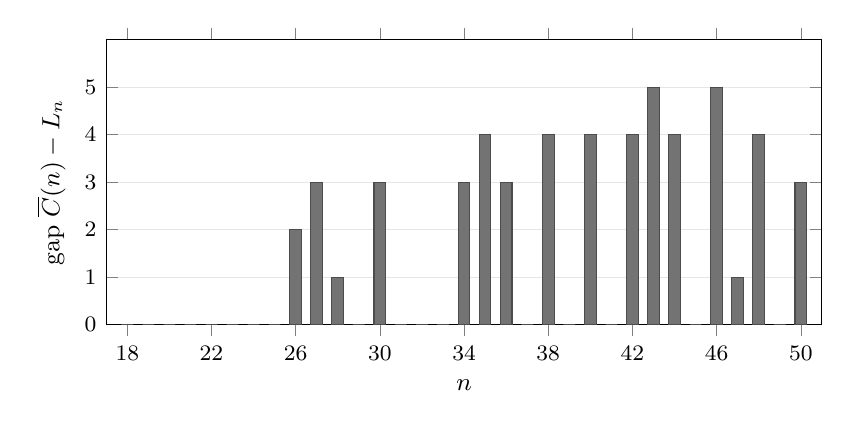
\begin{tikzpicture}
\begin{axis}[ybar,bar width=4.2pt,width=.88\textwidth,height=5.2cm,xlabel={$n$},
 ylabel={gap $\overline C(n)-L_n$},xmin=17,xmax=51,ymin=0,ymax=6,
 ytick={0,1,2,3,4,5},xtick={18,22,...,50},ymajorgrids=true,grid style={black!10},
 tick label style={font=\footnotesize},label style={font=\small}]
\addplot[fill=black!55,draw=black!70] coordinates {(18,0) (19,0) (20,0) (21,0) (22,0) (23,0) (24,0) (25,0) (26,2) (27,3) (28,1) (29,0) (30,3) (31,0) (32,0) (33,0) (34,3) (35,4) (36,3) (37,0) (38,4) (39,0) (40,4) (41,0) (42,4) (43,5) (44,4) (45,0) (46,5) (47,1) (48,4) (49,0) (50,3)};
\end{axis}
\end{tikzpicture}
